\chapter{Modular architecture}
\label{sec:ModularArchitecture}

Let's start with the definition of a modular architecture:
\largequote{Modular design or “modularity in design” is a design approach that subdivides a system into smaller parts called modules or skids that can be independently created and then used in different systems. A modular system is characterized by functional partitioning into discrete scalable and reusable modules, rigorous use of well-defined modular interfaces and making use of industry standards for interfaces. \cite{whatIsModularArchitecture}}

When looking at the famous architectures in software we have a few examples of non
modular architectures.

An example of such an architecture is the layered architecture. In the image below is shown how the architecture operates.

\begin{figure}[H]
	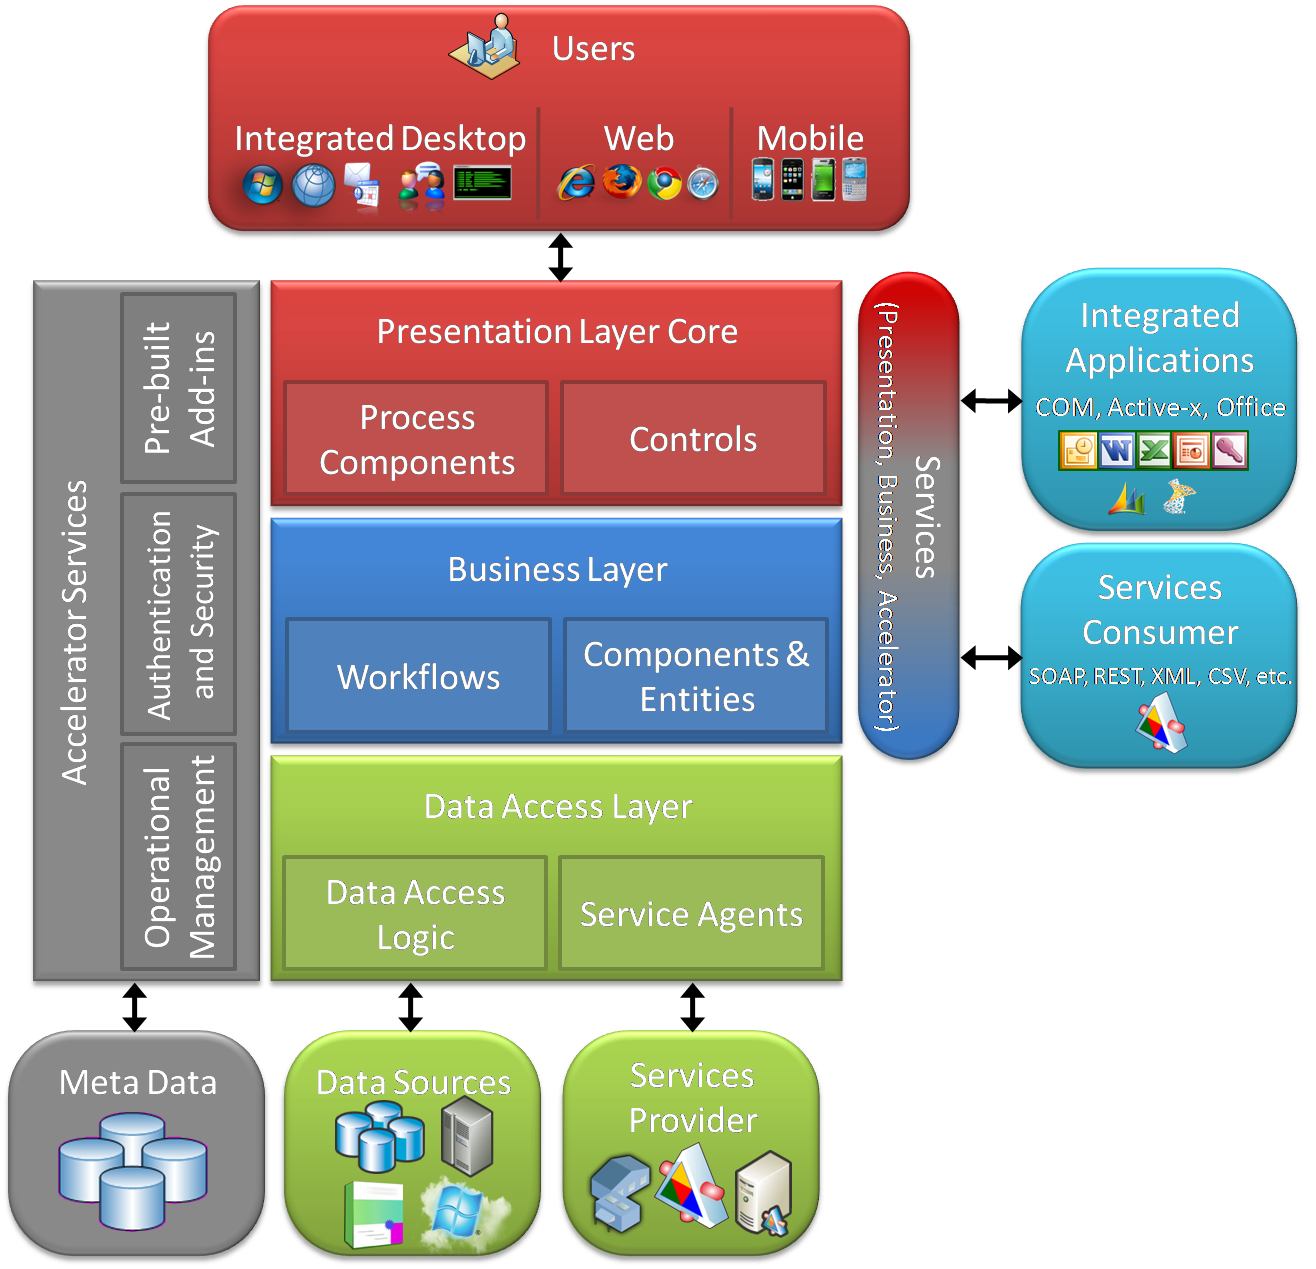
\includegraphics[width=\linewidth]{layered_architecture.png}
	\caption{Layered architecture \cite{layeredArchitecture}}
\end{figure}

As you can see in this image the architectures is layered based on responsibilities. This will conclude in each layer having its own purpose. As shown in the image the layers can talk with each other but they are intertwined. This means that a class or object in the presentation layer can talk to the same business layer object as another presentation layer class. Thus the objects are highly coupled.

So why is this architecture so different from a modular architecture? Well as the name suggests a modular architecture is based upon modules.

The definition of a module is:
\largequote{deployable, manageable, natively reusable, composable, stateless unit of software thatprovides a concise interface to consumers” \cite{moduleDefinition}}

This is eerily similar as the description of what we call building blocks in \fullref{sec:TheProblem}

\section{Architectures}
\label{sec:Architectures}

\subsection{Microservices}
If most software engineers in 2019 think of a modular software architecture the first architecture that comes up is microservices. In the last years microservices has seen a surge in usage. One of the most biggest companies that showed the effectiveness of microservices is Netflix.

\subsubsection{Definition}
The best way to describe a microservice is:
\largequote{A particular way of designing software applications as suites of independently
deployable services. \cite{microservicesDefinition}}

While there is no concrete definition of a microservice there are some characteristics that
every definition contains.
\begin{itemize}
        \item \textbf{Highly maintainable and testable} enables rapid and frequent development and deployment
        
        \item \textbf{Loosely coupled with other services:} enables a team to work independently the majority of time on their service(s) without being impacted by changes to other services and without affecting other services
        
        \item \textbf{Independently deployable:} enables a team to deploy their service without having to coordinate with other teams
        
        \item \textbf{Capable of being developed by a small team:} essential for high productivity by avoiding the high communication head of large teams \cite{microservicesCharactaristics}
\end{itemize}

Now that we have a clear understanding of what microservices are and which principles
they should follow we can pinpoint some best practices.

\subsubsection{Best practices}
The first best practices is to \textbf{create a seperate datastore} for each microservice. First of all not each datastore fits each service. It may be that a message service may get more efficiency from a NoSQL database and a user service from a SQL database. A benefit stemming from this is that microservices makes you think about each datastore used for each service and why that datastore is the correct one for that specific service \cite{microservicesNetflix}.

When creating a separate datastore for each service you run the risk of data inconsistency. For example, you have a user service which stores the user id. Also you have a message service which stores the message and the user id to whom the message is send. If the user id changes in the user service this should reflected in the message service. But with microservices this is not automatically the case because each service has its own datastore and therefore its no foreign keys that will be updated or give a warning.

Another best practices is \textbf{writing documentation} \cite{microservicesBestPractice} for each microservice. Most importantly about how they should be used and which interface it uses. For example, we create a new service next to our messaging and user service called file service which handles the files send in the messages. This service should know how to communicate with the message service and to make this easy for the new developers to connect to the existing services.

Another challenge with microservice is the \textbf{monitoring} \cite{microservicesBestPractice} of the services. Because it is not known how many services are online it is important to know when they are online and what they log. For example, our messaging service is used a lot and duplicate itself. This then means that the logging of the new service needs to be picked up by your monitoring system in order to view the whole picture of the running application.

\subsection{Miniservices}
Besides microservices which other architectures are there? One of the “new” ones is
miniservices. The reason new is between quotes is because most companies that implement
microservices actually implement miniservices. The difference between microservices and
miniservices is best described in the image below:

\begin{figure}[H]
	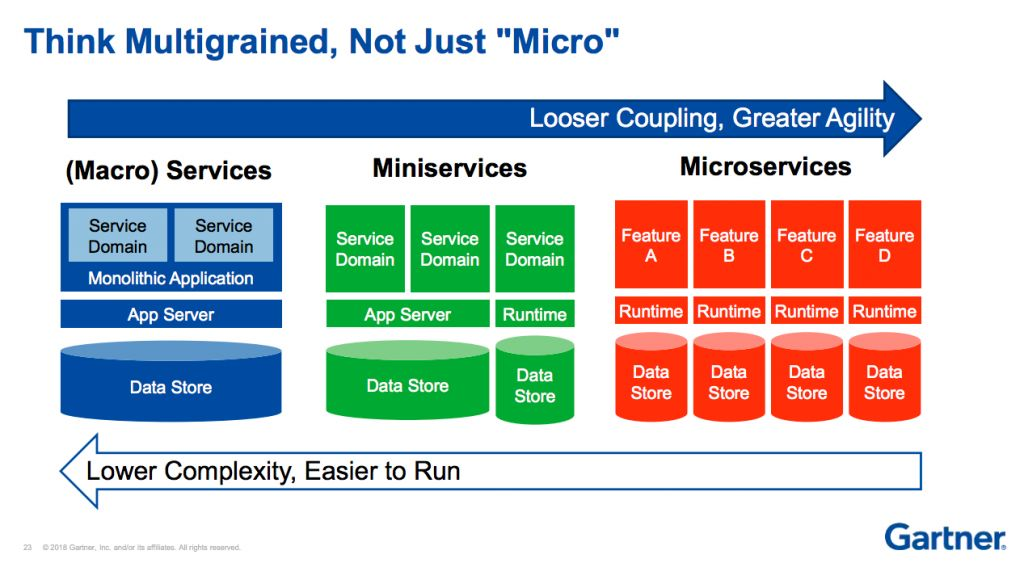
\includegraphics[width=\linewidth]{miniservices.png}
	\caption{Miniservices architecture \cite{miniservicesDefinition}}
\end{figure}

Miniservices are essentially an architecture based on breaking specific rules of microservices \cite{miniservicesOrigin}. As shown in the picture the biggest difference between microservices and miniservices are that microservices are actual features being decoupled and miniservice is about decoupling a domain of features.

What does this mean for the architecture? It means that each service may contain multiple features but all of the features should be linked to the same domain. Which means that the communication inside a service is way more fluent and needs less network design than microservices does.

Another divergence is that each microservice should have a separate datastore. This is not the case for miniservices. Every miniservice may be connected with the same datastore \cite{miniservicesDefinition}.

What are the advantages of miniservices over microservices? The most prominent answer is the complexity of the network architecture. With microservices every service is singled out. Which means no service knows about each other so the protocol in which the services speak can be different and may differ from service to service. Also with miniservices each service connects to the same database. Which makes it easier to do complex querying.

\subsection{Modular monolith}
\label{sec:ModularMonolith}

The main idea behind a modular monolith is preserving the idea of encapsulation but deploying it differently \cite{modularMonolithIdea}. Instead of deploying different services separately with each service having its own datastore, a module can be a library, plugin or namespace. This makes deploying way easier to manage but still having the modularity gotten from encapsulation. 

Just like with minservices each module will contain the functionalities of a single domain. But unlike the miniservices the modular monolith is compiled to one application instead of multiple.

\section{The comparison}
\label{sec:Comparison}

A good talk about modular monoliths \cite{modularMonolithTalk} shows that most of the time when thinking of architecture there are two extremes. The monoliths and the microservices. As shown in the image below:
\begin{figure}[H]
	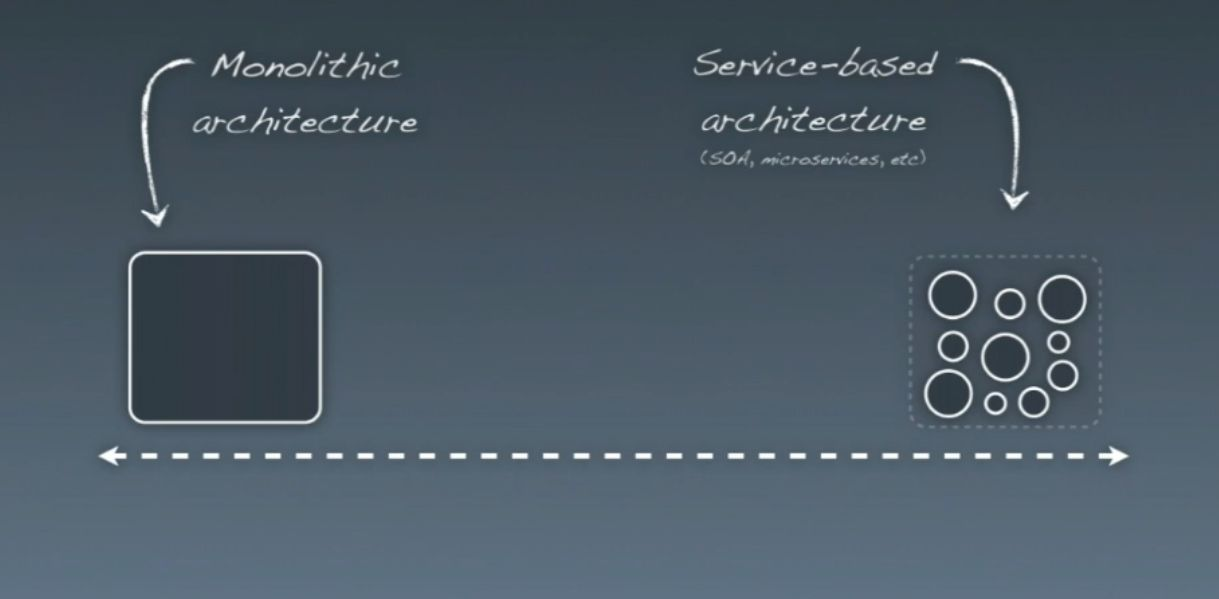
\includegraphics[width=\linewidth]{microservices-spectrum.png}
	\caption{Monolith, microservices spectrum \cite{modularMonolithTalk}}
\end{figure}

But this is not always the case as we showed in \fullref{sec:Architectures}.There are cases where microservices are the best choice and there are cases where miniservices or a modular monolith is the best choice. In this chapter I will compare the three architectures.

The question you should ask yourself is how important are these differences and why? This question can be coupled with the prioritization of the quality attributes as \fullref{sec:IsoRecap}

\section{Complexity}
\label{sec:Complexity}

Complexity always plays a role in choosing the right architecture. When looking at the three architectures shown \fullref{sec:Architectures} init is obvious that the complexity changes the smaller you go. Thus the most complex architecture is microservices and the least complex one is modular monolith. With miniservices right in the middle. But why?

In the image shown below there is an example of the microservice architecture. In this picture you can see that each service may have its own datastore but can also run on a different server. This means that each service needs to know in some way where the other services are located. This is called service discovery. Service instances have dynamically assigned network locations. Moreover, the set of service instances changes dynamically because of autoscaling, failures, and upgrades. Consequently, your client code needs to use a more elaborate service discovery mechanism \cite{serviceDiscovery}. This is also the case with miniservices.

\begin{figure}[H]
	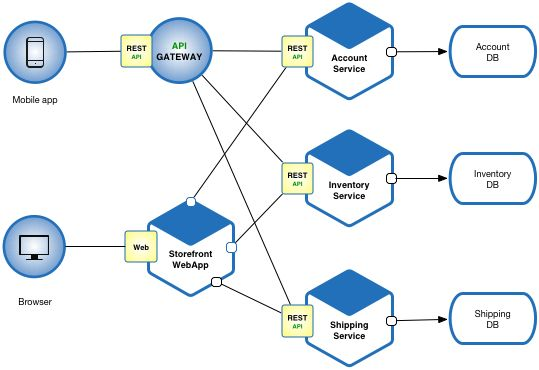
\includegraphics[width=\linewidth]{microservice-architecture.png}
	\caption{Microservice architecture}
\end{figure}

Even tho they can connect to a centralized datastore the services don’t have any knowledge of each other. In a monolith application there are no different services. The modules can talk with each other via functions and imports. This means that there is knowledge of the other modules.

The other thing that makes microservices especially complex is the splitted datastores. Because the database is splitted it can be hard to handle foreign keys or pointers to other data objects. This is because the datastore does not have a direct connection to this pointer. This problem of complexity is not prevalent amongst the miniservices and modular monolith because in these architectures the datastore is shared. But there is another problem with miniservices.

A service in the miniservices does not know what is in the other model only that there is another model. So somehow it should know how to get the remaining fields. This is the same problem you have with microservices and thus is very complex.

As mentioned above why and how is this important is crucial to ask. But let’s start linking this to quality attributes.

The quality attributes that are applicable to this attribute are:
\begin{itemize}
        \item \textbf{Maintainability:} The more complex an infrastructure and/or architecture is the more maintenance it requires.
        \item \textbf{Security:} Complexity always brings security issues with itself. This is especially the case with miniservices and microservices because of the service discovery.
\end{itemize}

\section{Technology}
\label{sec:Technology}

One of the most convincing arguments for choosing microservices is the freedom of choosing the technology. You can write the first service with Node.js and a MongoDB database and the next service with java and an elasticsearch datastore. This makes it really easy when switching technology or recruiting new developers.

Miniservices does have the benefit of choosing your own programming language but because all of the services talk with the same datastore the datastore technology is always the same.

Modular monoliths are the worst in this section. A modular monolith is stuck with the same technology as a programming language and with the datastore.

So which quality attributes are relevant to this attribute:
\begin{itemize}
        \item \textbf{Compatability:} The compatibility between technologies is extremely relevant when looking at the technology
        \item \textbf{Performance:} Because you can choose the technology for each service you can choose the language that creates the optimal performance for that specific service.
        \item \textbf{Porability:} The portability is very high because each service can be ported separately which makes it easier.
\end{itemize}

\section{Testing}
\label{sec:Testing}

It is known that testing plays a big role in creating reliable software. There are multiple types of testing \cite{testTypes}. Not all of them are useful for EFFE. That is why EFFE has created a list of tests it does on the current application. These are test types we will be looking at:

\begin{itemize}
        \item Unit tests
        \item Integration tests
        \item End-to-end tests
        \item Load tests
\end{itemize}

\subsection{Unit tests}
\label{sec:UnitTests}

\begin{enumerate}
        \item Microservices
        \item Miniservices
        \item Modular monolith
\end{enumerate}

This is because especially in a microservice because each function is its own service the functions are really easy to test. Because miniservices are domain based it takes a bit more effort to test the whole service but it is easier than the modular monolith. This is because the modular monolith is a bit tighter coupled than the miniservice.

\subsection{Integration tests}

\begin{enumerate}
        \item Miniservices
        \item Modular monolith
        \item Microservices
\end{enumerate}

Because the modular monolith contains all its services it is easy to test how they work together. This can even be done with unittesting. For the miniservices and microservices it is way more difficult. The reasoning behind this is the complexity of the service discovery. To test for example two services you need to setup the service discovery. With each service that needs to be tested it will become harder to test it because more services need to be discovered. A integration test with microservices may call 6 different services. But with miniservices it may be less if the functions that are called are in the same domain. This is why microservices gets the last place in this type of testing.

\subsection{End-to-end tests}

\begin{enumerate}
        \item Miniservices
        \item Modular monolith
        \item Microservices
\end{enumerate}

As seen with the previous test types the same problem occurs. A function that is called may need multiple microservices or miniservices called.

\subsection{Load tests}

No difference

All of the architectures are equal when it comes to load testing. This is because load testing is done on a live site. This does not mean it has to be done on production although it can be.

\subsection{Conclusion}

So what are the quality attributes that testing influences:

\begin{itemize}
        \item \textbf{Maintainability:} Maintainability is about effectiveness and efficiency. Both can be measured with load testing. It is an important quality attribute but because load testing is equal for all we don’t consider this one

        \item \textbf{Compatibility:} Almost all of the test types look at if the code works and will fail if it changes. This concludes in looking at backwards compatibility and a check on it. Testing has a very high impact on this quality attribute.
 
        \item \textbf{Functional sustainability:} This is where testing started. Writing unit tests to be sure the functionality hasn’t changes.
 
        \item \textbf{Performance:} With load testing performance will be tested but as with maintainability this won’t be taken in consideration.
 
        \item \textbf{Usability:} End-to-end testing is specifically made for testing this and check if the usability is still the same. 
\end{itemize}

\section{Costs}
\label{sec:Costs}

Because EFFE is a startup costs are very important. EFFE does not have the steady money flow of a more mature company. Even though EFFE has gotten \$20.000,- for Google cloud platform for one year we need to consider what happens after that year.

There are two parts on how costs are created for software. The first one contains the price of development and the second one is the price of hosting.

Right now EFFE employs one software engineer, Jessie Liauw A Fong. But he is also the co-founder so there is no money yet to be made by Jessie. This is because all the money EFFE makes goes right back into EFFE. But as mentioned before we should still consider what would happen if EFFE would hire more software engineers.

Development time and understanding the code go hand in hand. When you don’t understand the code you can’t develop. So how do these architectures hold considering development time and understanding the code?

Microservices as mentioned before is a very complex architecture but when developing is one of the easiest ones. Because each function is its own service, creating a service is really easy. There is not a lot of code in one function and therefore easy to understand.

Minservices and a modular monolith are in the same situation the code can be more complex because they need to talk to other services or modules but there is also a lot of code in one service or module. Therefore understanding the code and thus the developing time become larger.

But how big of a difference is there in this? Not much depending on your architecture. If your miniservices and modular monolith are structured in such a way that is logical it should not matter.

But when looking at the infrastructure there is a complete 180. Modular monolith is by far the least expensive architecture. Because the application can run on one server without the expense of server discovery it can be run on a server that costs \$5,- a month \cite{digitalOcean}. But the tricky parts comes when talking about interchangeability. What happens if a company wants a building block changed slightly only for them. If they are willing to pay for it it means that there needs to be a whole new server because the application is build on its own. When we have 5 clients who want this and 5 clients that run on the standard version we would have to run it on 6 servers which would be \$30 dollars on the cheapest server which is not expensive at all.

Microservices and miniservices are the opposite side with microservice standing out more. These services require server discovery as mentioned before. There are open source server discovery services such as consul but those also need a seperate server. But server discovery is not the most expensive part. The most expensive part is a combination of having multiple services running on different servers that can autoscale. This means that we have less knowledge about our spendings beforehand.

How can you deploy multiple services automatically. There are some amazing services for this. The most known are Kubernetes, Nomad and Docker swarm. These services however cost \$40,- per month with the minimum requirements. And that is if you only have three instances of such a service running. The cost of the servers and the orchestrator can ramp up quickly.

The quality attribute that is most affected by the cost is the maintainability.This is purely because if the infrastructure is this expensive there would be no money to maintain it.

\subsection{Conclusion}
Thus when looking at development time vs infrastructure costs there is a lot to say for modular monoliths. Because even tho the development time is a bit slower for modular monoliths the infrastructure is way cheaper than miniservices or microservices.

\section{Scalability}
\label{sec:Scalability}

It wouldn’t be fair to compare these architectures without taking a look at scalability. This is where microservices shine. This is where microservices are made for. Microservices are made for horizontal scaling.

Vertical scaling is when you are adding hardware resources to a server. For example adding 4GB of ram to a server. Horizontal scaling is when adding more instances of the service. This can be on multiple servers \cite{microservicesMultipleServer}.

As mentioned before microservices is created for horizontal scaling. When a service suddenly gets a lot of traffic the service can autoscale itself. This can be done rather easily because the service itself is so small. This is also why it is harder with miniservices and even harder with modular monolith. Because when deploying a new version of those instances you need to deploy in modular monoliths part the whole application.

When is scalability important? Well when talking about \textbf{performance}. This is also the quality attribute that is affected by scalability. When a server is going above a certain threshold it can duplicate itself and can now split the traffic along the new instance.

\section{Frontend}
\label{sec:Frontend}

So until now most of the comparison were for backend or did also apply to frontend but it was not mentioned. When looking at the architecture there is one that stands out as easily adapted for frontend and that is modular monolith. This is because it will still be compiled to one application.

First of all let’s define what EFFE considered for frontend. Right now we use Vue to create a single page application. But this does not mean other frontend frameworks are not considered.

When looking at microservices in the backend there is a similar phenomenon in the frontend called micro-frontend or micro-apps \cite{microFrontends}. But there is one problem that persists with this solution ant that is the sharing of ui elements. You can share them between services but that would mean each service would use the same language and need to be deployed all together if one of those ui elements change. Therefore this is not a solution. An talk about micro-apps (microservices frontend) gave a convincing story about why you should switch to them \cite{frontendMicroservices}. But when asked about the UI elements there was no answer to this question.

What happens in the current implementations of microservices and miniservices. The answer might surprise you. There is no such thing as microapps for big application. Most of them is just one single code base.

Concluding that for frontend there is only one possibility when looking at modularity and that is modular monolith.

\section{Recap}

There is a lot of articles written about monoliths vs microservices. In the end minservices has some of the benefits and cons of both.

This is a recap of what is discussed in \fullref{sec:ModularArchitecture}. As mentioned in \fullref{sec:Comparison} we would look at the quality attributes and how they matched up per architecture.

\fullref{sec:Complexity} talks about the complexity and how it can influence the whole project in its whole. The one that came out best was modular monolith and the quality attributes that were applicable where \textbf{maintainability} and \textbf{security}.

\fullref{sec:Technology} microservices came out on top with flying colors. With miniservices following and modular monolith as a obvious last. The quality attributes that are influenced by technology are \textbf{,ompatibility}, \textbf{performance} and \textbf{portability}

\fullref{sec:Testing} was by far the most contested section with no clear winner. But if you looked at the types of tests that were considered (unit, integration, end-to-end and load testing) modular monolith ended with the best result with miniservices again in the middle and microservices ending last. The quality attributes for testing are \textbf{maintainability}, \textbf{compatibility}, \textbf{funtional sustiainability}, \textbf{performance} and \textbf{sustainability}

\fullref{sec:Costs} the clear winner in this section was modular monolith with miniservices following and microservices at a obvious last place. The quality attributes affected by the cost is \textbf{maintainability}

\fullref{sec:Scalability} the obvious winner was microservices. In second place was miniservices andlast was modular monolith. The quality attribute applicable is \textbf{performance}.

\fullref{sec:Frontend} eventually there was only one architecture that actually made sense for frontend and that was the modular monolith.

\section{Conclusion}

The architecture that fits EFFE best is the modular monolith. The chapters where modular monolith took the first place by far were also the ones that influenced the quality attribute \textbf{maintainability} the most. As sorted in \fullref{sec:IsoRecap} \textbf{maintainability} is by far most important to EFFE. EFFE also does not have a lot of money as mentioned in \fullref{sec:Costs} Thus costs play a big part in this decision as well. Last of all the modular monolith architecture is especially good for small teams and that is a perfect description of the software team of EFFE since it exists out of one person.

Microservices have the clear distinction of winning the race on technology and scalability but this is not where the focus lays. Though technology will offer some of our focusses is 24does not compete with the main focus that the modular monolith architecture touches on and the cons do not outweigh the pros.

So why not miniservices? Miniservices is a mixture of modular monolith and microservices and it does take some good parts of the both architectures but also some cons of both architectures. The biggest con here is the complexity of the datastore. Even though the same datastore is shared over the services you cannot get everything in one request. As explained in \fullref{sec:Complexity}.

And last of all both microservices and miniservices cost to much for EFFE at this stage of the company. 
